% pdflatex -shell-escape template_cdc.tex

\documentclass[a4paper,oneside]{article}

\usepackage[frenchb]{babel}
\usepackage[utf8]{inputenc}
\usepackage[T1]{fontenc}
\usepackage{graphicx}
\usepackage{amssymb} 
\usepackage{amsmath}
\usepackage{hyperref}
\usepackage{fullpage}
\usepackage{epstopdf}


%%%%%%%%%%%%%%%%%%%%%%%%%

\newcommand{\mytitle}{Projet Bataille Navale - Cahier des charges}
\title{\mytitle } 

%%%%%%%%%%%%%%%%%%%%%%%%%

\makeatletter

\usepackage{fancyhdr}
\pagestyle{fancyplain}
\fancyhf{}
\renewcommand{\headrulewidth}{0pt}
\renewcommand{\footrulewidth}{0.5pt}
\lfoot{\mytitle}
\cfoot{\@date}
\rfoot{page \thepage / \pageref{fin}}

\author{Alexandre Tholliez - Thomas Prunier - Quentin Coloos - Benoît Verhaghe}

\date{29 mai 2017}


%%%%%%%%%%%%%%%%%%%%%%%%%


\begin{document}

\maketitle

\thispagestyle{fancyplain}


%%%%%%%%%%%%%%%%%%%%%%%%%

\section{Renseignements}

\paragraph{Nom du projet :}
Bataille Navale

\paragraph{Objet :}
Développement d'un jeu de bataille navale avec création d'une IA

\paragraph{Maître d'ouvrage :}
Alexandre Tholliez - Thomas Prunier - Quentin Coloos - Benoît Verhaghe

\paragraph{Maître d'oeuvre : }
Alexandre Tholliez - Thomas Prunier - Quentin Coloos - Benoît Verhaghe

\paragraph{Date de début :}
29 mai 2017

\paragraph{Date de fin :}
18 juin 2017


%%%%%%%%%%%%%%%%%%%%%%%%%

\newpage

\section{Définition du besoin}

\paragraph{Contexte général\\}
Nous voulons ici mettre en pratique les notions qui nous ont été enseignées pendant nos trois années de licence.
Notre choix s'est porté sur la création d'un jeu utilisant une Intelligence Artificielle.
Il combine à la fois la programmation orienté objet, la notion d'IA et le génie logiciel avec l'utilisation de
Github.


\paragraph{Besoins et priorités\\}
Le besoin principal est d'avoir une IA fonctionnelle et différents niveaux de difficultés.
Nous voulons également implémenter la possibilité de faire du joueur contre joueur mais
également du IA vs IA.
Il s'avère essentiel d'avoir une interface graphique simple et intuitive.

%%%%%%%%%%%%%%%%%%%%%%%%%

\newpage

\section{Spécifications}

\begin{itemize}
    \item jeu fonctionnant sur toute machine avec une distribution linux
    \item fonctionnalités du jeu de bataille navale :
        \begin{itemize}
            \item Choisir le mode de jeu
            \begin{itemize}
            	\item Joueur contre Joueur
            	\item Joueur contre IA
            	\item IA contre IA
            \end{itemize}
            \item Jouer une partie
            \begin{itemize}
            	\item Initialisation du plateau de jeu
            	\item Placement des bateaux
            	\item Jouer un coup
            	\item Vérification du coup (touché ou raté ou coulé ou victoire)
            	\item Jouer coup suivant tant que pas de victoire
            \end{itemize}
        \end{itemize}
    \item interface utilisateur :
        \begin{itemize}
            \item interface graphique
            \item affichage du plateau avec les tirs et bateaux du joueur
        \end{itemize}
    \item performances demandées :
        \begin{itemize}
            \item vérification de la légalité des coups
            \item IA performante en fonction de la difficulté
        \end{itemize}
\end{itemize}


%%%%%%%%%%%%%%%%%%%%%%%%%

\newpage

\appendix

\section{Livrables}

\begin{itemize}
    \item logiciel déployé sur machine utilisant linux
    \item code source documenté sous doxygen
    \item manuel utilisateur sous sphinx
\end{itemize}

\section{Diagrammes de cas d'utilisation}

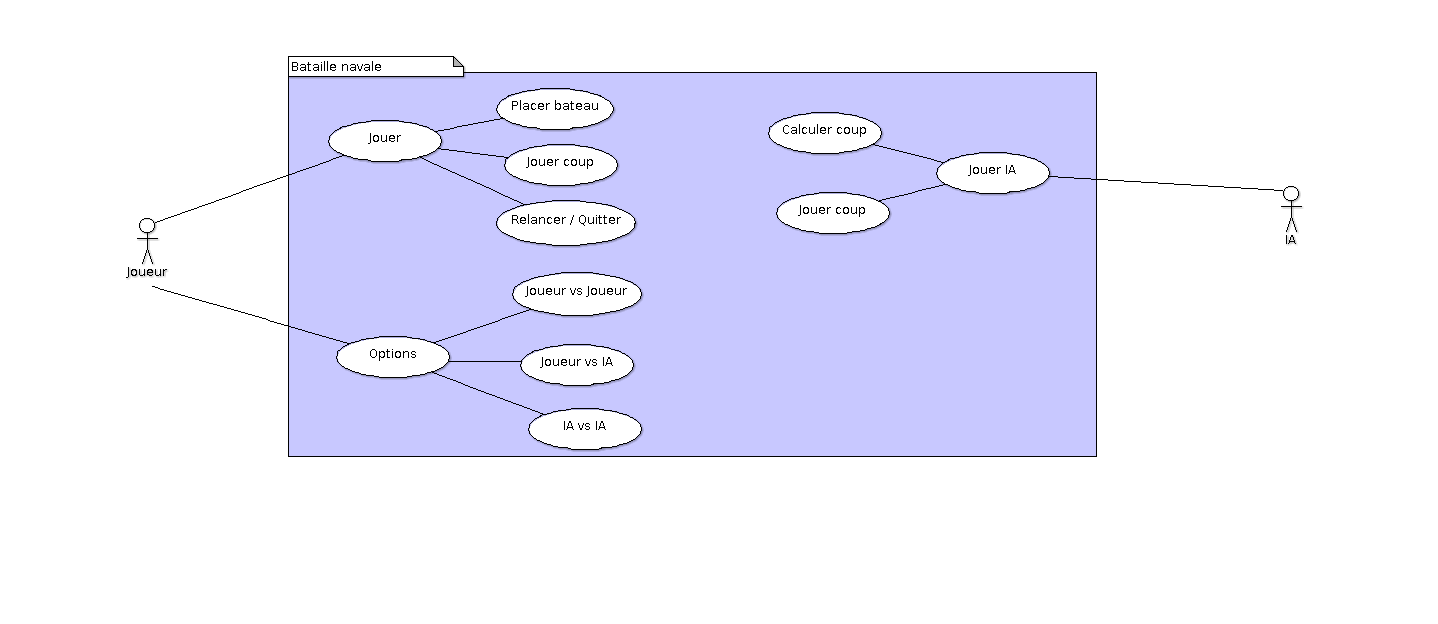
\includegraphics[width=19cm]{diagramme.png}




\section{Maquettes}

\paragraph{Interface Selection\\}

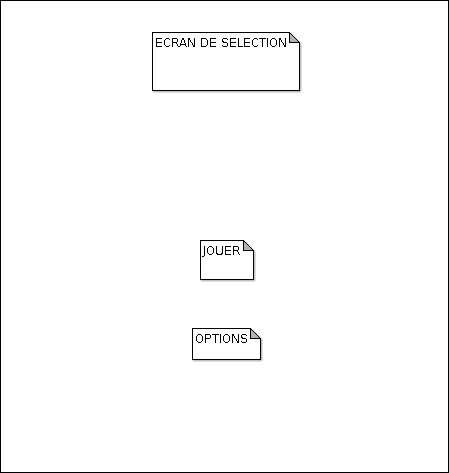
\includegraphics[width=9cm]{maquette_selection.png}



\paragraph{Interface Options\\}

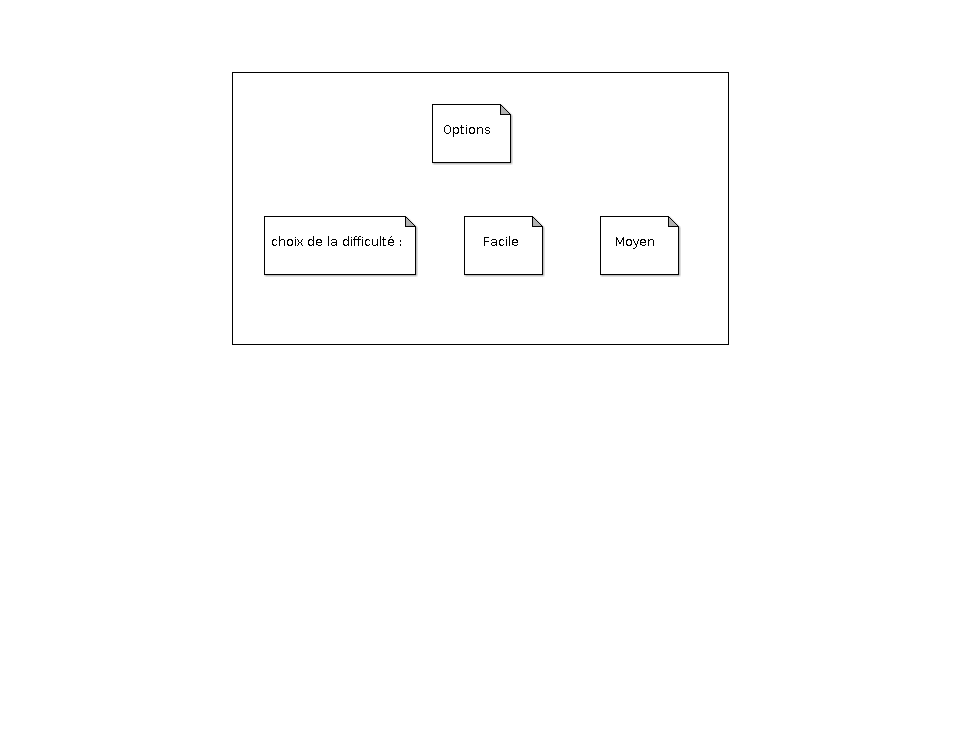
\includegraphics[width=9cm]{maquette_options.png}



\paragraph{Interface Jeu\\}

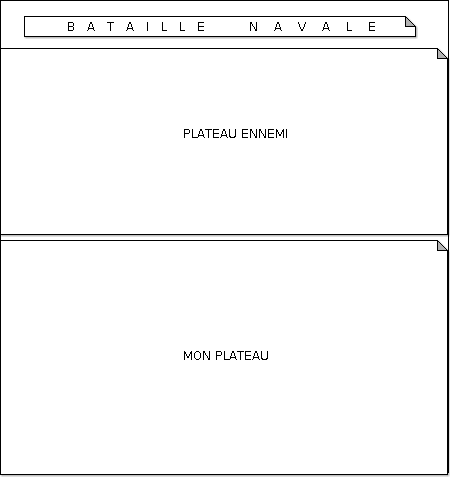
\includegraphics[width=9cm]{maquette_jeu.png}




%\section{Planning prévisionnel}

%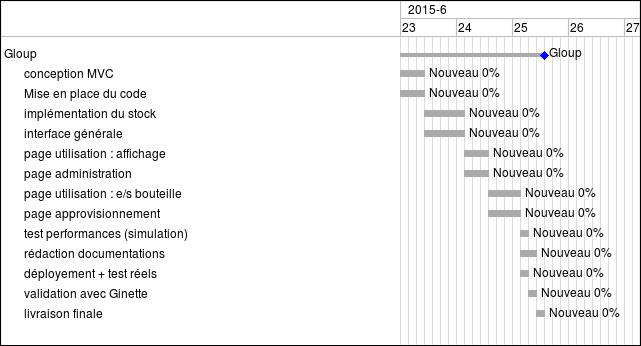
\includegraphics[width=13cm]{cdc_gantt.png}


%\section{...}


%%%%%%%%%%%%%%%%%%%%%%%%%

\label{fin}

\end{document}


